%% go to the website http://en.wikibooks.org/wiki/LaTeX For Help 
\documentclass[11.5pt]{article}
%Math Related Packages
\usepackage{mathtools}
\usepackage{amsmath}
\usepackage{amsfonts}
\usepackage{amssymb}
\usepackage{relsize}
% Pseudocode Packages
\usepackage{algorithm}
\usepackage{algpseudocode}
\usepackage[colorinlistoftodos]{todonotes}
% Automata/Graph Packages
\usepackage{tikz}
\usepackage{pgf}
\usetikzlibrary{arrows,automata}
\usepackage[latin1]{inputenc}
\usetikzlibrary{automata,positioning}
%%%Formatting Options for Pages
%\usepackage[a4paper,left=2cm,right=2cm]{geometry} %Change Margins
\usepackage[colorlinks=true, allcolors=blue]{hyperref} % adds hyperlinks
\usepackage{listings}
\usepackage{multicol}
\usepackage{perpage}
\MakePerPage{footnote}
%%%Graphics Packages and Caption Tools
\usepackage{graphicx}
\usepackage{fullpage}
\newcounter{Figure} 
\setcounter{Figure}{1}
\usepackage{slashbox}
\usepackage{ulem}
\usepackage{csvsimple}
%%%Colors Package with Custom Defined Colors
\usepackage{color}
\usepackage{colortbl}
\definecolor{Gray}{gray}{0.9}
\definecolor{codegreen}{rgb}{0,0.6,.2}
\definecolor{codegray}{rgb}{0.5,0.5,0.5}
\definecolor{codepurple}{rgb}{0.58,0,0.82}
\definecolor{backcolor}{rgb}{0.94,0.94,1}
\definecolor{light-gray}{gray}{0.55}
%%Custom Functions and Commands
\newcommand\indentFour{\indent\indent\indent\indent}
\newcommand\indentThree{\indent\indent\indent}
\newcommand\indentTwo{\indent\indent}
\newcommand\tab{\ \ \ }
\newcommand\proof{\setcounter{equation}{0}\hfill\fbox{\rule{.02in}{0pt}\rule[0ex]{0pt}{.5ex}}}
%%Color Commands
\newcommand\BLK{\color{black}}
\newcommand\GRY{\color{Gray}}
\newcommand\BLU{\color{blue}}
\newcommand\blu{\color{CornflowerBlue}}
\newcommand\RED{\color{red}}
\newcommand\red{\color{RubineRed}}
\newcommand\ORG{\color{BurntOrange}}
\newcommand\org{\color{Peach}}
\newcommand\GRN{\color{ForestGreen}}
\newcommand\grn{\color{LimeGreen}}
\newcommand\PRP{\color{RoyalPurple}}
\newcommand\prp{\color{DarkOrchid}}
%%Math Commands
\newcommand{\Lbra}{\left\langle}
\newcommand{\Rbra}{\right|}
\newcommand{\Rket}{\right\rangle}
\newcommand{\Lket}{\left|}
\newcommand{\bra}[1]{\Lbra #1 \Rbra}
\newcommand{\ket}[1]{\Lket #1 \Rket}
\newcommand{\braket}[1]{\Lbra #1 \Rket}
\newcommand{\Exists}{\ \exists \ }
\newcommand{\Forall}{\ \forall \ }
\newcommand{\abs}[1]{\left| #1 \right|}
\newcommand{\Frac}[2]{\left(\frac{#1}{#2}\right)}
\newcommand{\Mat}[1]{\left[\begin{matrix} #1 \end{matrix}\right]}
\newcommand{\vhi}{\varphi}
\newcommand{\R}{\ \mathbb{R}}
\newcommand{\C}{\ \mathbb{C}}
\newcommand{\N}{\ \mathbb{N}}
\newcommand{\Z}{\ \mathbb{Z}}
\newcommand{\I}{\ \mathbb{R/Q}}
\newcommand{\x}{\mathrm{x}}
\newcommand{\mbf}[1]{\mathbf{#1}}
\newcommand{\Dpart}[2]{\frac{\partial #1}{\partial #2}}
\DeclarePairedDelimiter{\ceil}{\lceil}{\rceil}
\newcommand{\U}{\underline}
%Numbering
\newcounter{graphics}
\newcounter{tables}
%For coding
\lstdefinestyle{small}{
    backgroundcolor=\color{backcolor},   
    commentstyle=\color{codegreen},
    keywordstyle=\color{blue},
    numberstyle=\tiny\color{codegray},
    stringstyle=\color{codepurple},
    basicstyle=\footnotesize,
    breakatwhitespace=false,         
    breaklines=false,                 
    captionpos=b,                    
    keepspaces=false,                 
    numbers=left,                    
    numbersep=5pt,                  
    showspaces=false,                
    showstringspaces=false,
    showtabs=false,                  
    tabsize=4
}
%\lstinputlisting[language=Matlab]{cub_spline.m} %Use this to add code
\renewcommand{\abstractname}{Abstract}
\begin{document}
\title{MAT 125B - Homework \# 7}
\author{Douglas Sherman \#: 913348406}
\date{January 27th, 2017}
\maketitle
\rule{\textwidth}{1pt}
\lstset{style=small} %set code style, see preamble


To test that the numerical computations are returning accurate numerical approximations, we test on a variety of known solutions. Moreover, by ensuring that the error does descrease according to the expected local truncation error by Taylor's theorem for each method, we can instill more confidence in the result. Consider the following initial value problems (IVP).
\begin{center}
\begin{tabular}{|c|c|c|}
\hline
	$\mbf{y'=f(t,y(t))}$&$\mbf{y(t_0) = y_0}$	&$\mbf{y(t)}$	\\
\hline
	$y' = 2y(t)/t$&$y(-1)=3$	&$y(t) = 3t^2$		\\
\hline
$y' = 2t^2y(t)$	&$y(0) = 2$	&$y(t)=2e^{2t^3/3}$		\\
	\hline
	$y' = y(t)^t$	&$y(-2) = 1.5874$	&$y(t)=(10-t(t - 1))^{1/(1-t)}$		\\
	\hline
	$y' = ty(t)^2$	&$y(-1) = 1$	&$y(t)=2/(3 - t^2)$		\\
	\hline
\end{tabular}\\
\begin{scriptsize}
{\bf \stepcounter{tables}\arabic{tables}.} Selection of known Initial Value Problems
\end{scriptsize}
\end{center}
Once the known IVPs were determined we tested the accuracy of different numerical approximation including Euler's Method, the midpoint method, and Heun's Method. The Following illustrates the accuracy for the various number of intervals $n$. 

\begin{center}
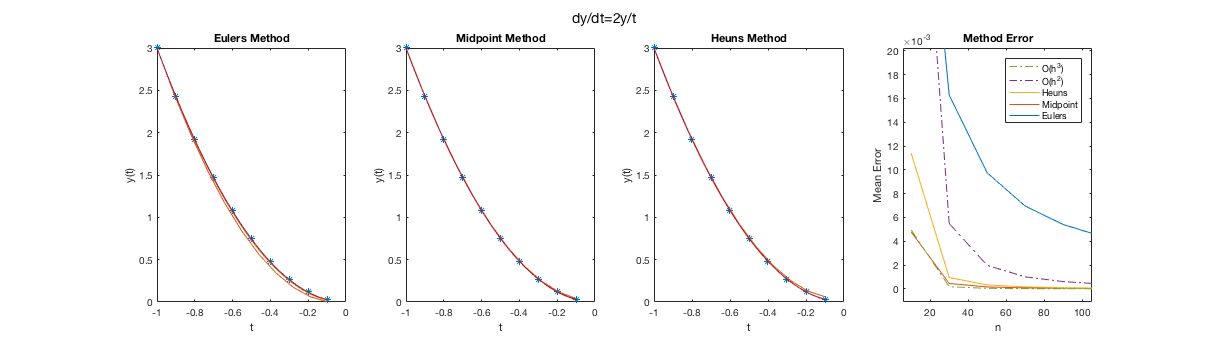
\includegraphics[width = 6in]{1st.png}\\
\begin{scriptsize}
{\bf \stepcounter{graphics}\arabic{graphics}.} Comparison of Multiple Methods for $y' = 2y/t$
\end{scriptsize}
\end{center}
\begin{center}
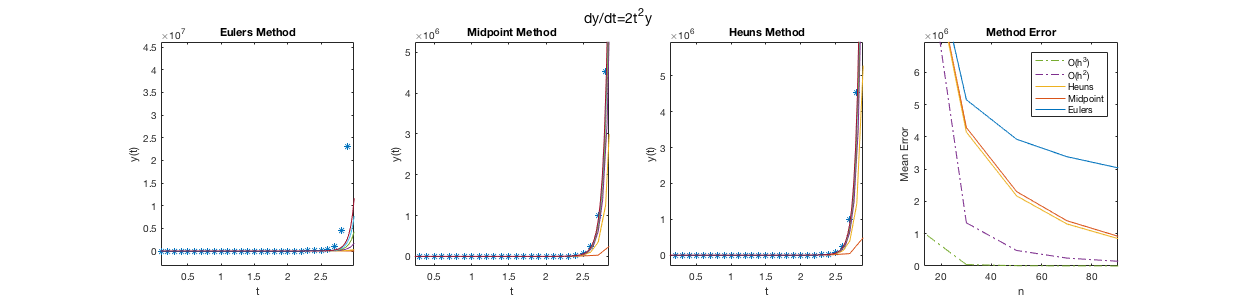
\includegraphics[width = 6in]{2nd.png}\\
\begin{scriptsize}
{\bf \stepcounter{graphics}\arabic{graphics}.} Comparison of Multiple Methods for $y' = 2t^2y$
\end{scriptsize}
\end{center}
\begin{center}
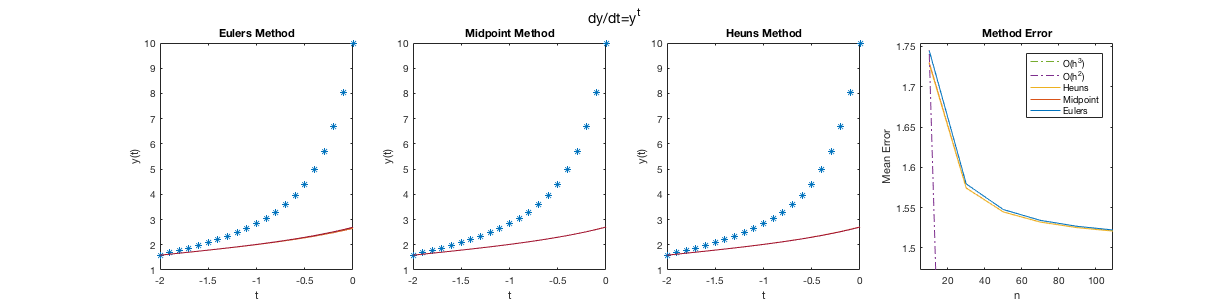
\includegraphics[width = 6in]{3rd.png}\\
\begin{scriptsize}
{\bf \stepcounter{graphics}\arabic{graphics}.} Comparison of Multiple Methods for $y' = y^t$
\end{scriptsize}
\end{center}
\begin{center}
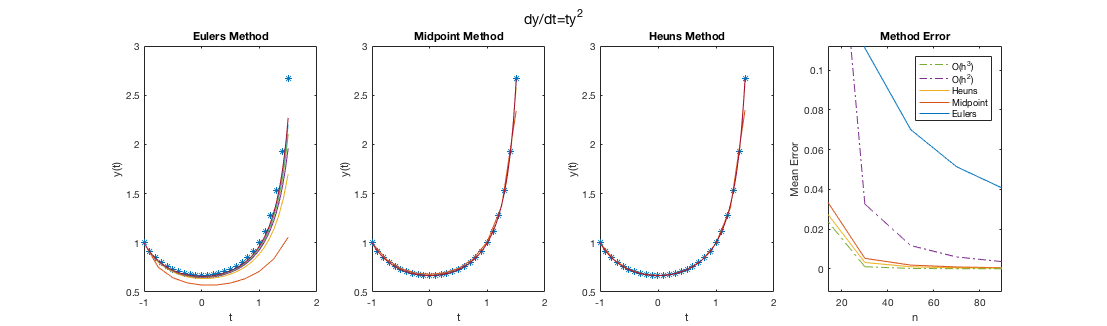
\includegraphics[width = 6in]{4th.png}\\
\begin{scriptsize}
{\bf \stepcounter{graphics}\arabic{graphics}.} Comparison of Multiple Methods for $y' = ty^2$
\end{scriptsize}
\end{center}


\end{document}